\section*{Аннотация}
\addcontentsline{toc}{section}{Аннотация}

В курсовом проекте описан процесс разработки участка для упаковки поддонов с ящиками крепёжных запчастей, используемых в промышленности и строительстве. Необходимое оборудование размещается по ходу технологического процесса. Выбрана оптимальная информационная система и система управления. Разработан алгоритм управления технологическим оборудованием и предложена программа для системы управления.

\section*{Введение}
\addcontentsline{toc}{section}{Введение}

Согласно статистике, среди многих случаев ущерба, которые можно было бы предотвратить, например, при международных перевозках, две трети составляют те, которые связаны с упаковкой. Поэтому часто в условия договора купли-продажи сторонами обычно вносятся специальные положения, содержащие требования относительно вида и характера тары и упаковки, ее качества и размеров. Важность этого момента бесспорна. Особенно в случаях, когда продукция поставляется не только на внутренний рынок, но рассчитана и на зарубежного потребителя. 

Стоимость готовой продукции, как правило, является наивысшей в момент завершения ее изготовления. Однако реализовать эту стоимость в полной мере можно лишь в том случае, если продукт в целости и сохранности поступит к покупателю. А ведь путь к нему может быть довольно длинным, как во времени, так и в пространстве. И, конечно, на этом пути встречаются обстоятельства, которые негативно влияют на сохранность продукта, причиняя ему иногда существенный ущерб. 

В последние годы требования к упаковке во многих странах резко возросли. Сегодня упаковочные материалы, способы и виды упаковки во многом влияют на объемы продаж и на мировую торговлю в целом, и в итоге --- на положение каждой отдельной компании на рынке. Улучшая упаковку, компания повышает свою конкурентоспособность на рынке. Однако многие компании стоят перед выбором: улучшение качества упаковки и стабильности груза в ущерб производительности или наоборот, увеличение производительности при некотором снижении требований к упаковке. 

Однако уже давно существуют решения, позволяющие сохранять, а во многих случаях и улучшать качество упаковываемого груза при увеличении упаковываемого в единицу времени товара --- это полностью автоматизированное оборудование по формированию и упаковке грузов. Ко всему прочему, автоматическое оборудование практически исключает из производственного процесса человеческий фактор, что положительным образом сказывается на внешнем виде упаковки, большей его стабильности и лучшей защите от капризов погоды. 

Но и это не самое главное, важно то, что автоматическое оборудование позволяет получить фиксированную стоимость упаковки на каждую коробку, каждый поддон и, соответственно, дает возможность постоянного и экономичного расхода используемого упаковочного материала. При использовании ручного или полуавтоматического способа упаковки, оператор часто применяет «еще один» слой пленки к каждому поддону, чтобы быть уверенным в стабильности упаковки, и увеличивает тем самым затраты на упаковку каждого поддона~\cite{stroi:upakovka}.

\section{Обзор существующих технологий упаковки}

\subsection*{Автоматические палетайзеры (палетоукладчики)}
Палетайзер формирует на столе слой, например, коробов с продукцией, поступающих с конвейера, и укладывает его на палету слой за слоем в соответствии с заданными параметрами. Оборудование по укладке продукта на палету незаменимо в случаях, когда необходимо упаковывать большое количество продукции в единицу времени, сформировать высокую палету или когда груз имеет большой вес.

Основные типы автоматических палетайзеров:

\begin{itemize}
    \item автоматические палетайзеры с послойным формированием палеты с помощью толкателя; 
    \item автоматические палетайзеры с формированием палеты с помощью манипулятора. 
\end{itemize}

Технологически палетайзер располагается между производственной линией предприятия и линией для упаковки палет (например, автоматической линией для упаковки палет стретч пленкой).

Производительность палетайзера зависит от мощности производственной линии предприятия. 

В зависимости от того, сколько единиц продукции (коробов, мешков и т. д.) в единицу времени сходит с производственной линии, и выбираются показатели линии для укладки продукта на палету.


\subsection*{Автоматические линии для упаковки палет стягивающими лентами (strap)}

Экономическая выгода от использования автоматических линий для упаковки палет состоит в том, что они позволяют получить фиксированную стоимость упаковки на каждую палету с грузом и, соответственно, дают возможность оценки постоянного расхода используемого упаковочного материала. 

Автоматические линии для упаковки палет стягивающими лентами (strap) предназначены для скрепления транспортных упаковок любого типа и закрепления их на палете с помощью стягивающей ленты (strap).

Оборудование используется для упаковки строительных и отделочных материалов (керамической плитки, шифера, кирпича, бордюрного камня, профиля, блоков, гипсокартона и пр.), продуктов черной и цветной металлургии (труб, кабеля, арматуры, листового проката и пр.), пиломатериалов, ДСП, паркета, мебели, полиграфической и картонажной продукции и пр. 

Технология работы автоматических линий для упаковки палет стягивающими лентами (strap):

Палета с грузом по конвейерам поступает в рабочую область машины. Затем при помощи арки лента оборачивается вокруг упаковываемого груза. В соответствии с заданными параметрами цикла машина регулирует натяжение, запаивает и обрезает ленту. 

\begin{figure}[ht]
    \subfloat[]{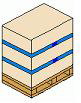
\includegraphics[width=.3\linewidth]{Figures/tight1.png}}
    \qquad
    \subfloat[]{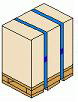
\includegraphics[width=.3\linewidth]{Figures/tight2.png}}
    \caption{Виды обвязки стягивающей лентой (а) горизонтальная; (б) вертикальная}
    \label{fig:tight}
\end{figure}

Производительность автоматических линий зависит от количества обвязок лентой одной палеты с грузом и типа используемой ленты. Количество обвязок задается программно. Время цикла одной обвязки --- 1--2,5 секунды.

Универсальные возможности автоматических линий для упаковки палет стягивающими лентами (strap):

\begin{itemize}
    \item интеграция в производственную линию предприятия; 
    \item сила натяжения ленты регулируемая (от 0 до 700 кг) – в зависимости от типа упаковываемого груза; 
    \item скрепление груза в горизонтальном или вертикальном направлении; 
    \item высокая сила натяжения и прочность соединения ленты; 
    \item работа с лентой любой ширины без специальных настроек ;
    \item возможность установки устройства уплотнения груза с четырех сторон;
    \item скорость натяжения ленты вокруг груза перед запайкой (0,05 – 0,25 м/сек) ниже скорости протяжки ленты (0,7 – 4,8 м/сек), что позволяет избежать повреждения краев; 
    \item комплектация арками любых размеров в зависимости от типа упаковываемого груза (для упаковки грузов необходимого размера); 
    \item дополнительная установка двойной обвязочной арки для обвязки груза одновременно в двух местах и увеличения производительности. 
\end{itemize}

Расходные материалы --- полипропиленовая или полиэстеровая страп лента, в том числе с нанесением печати: ширина --- 8--19 мм, толщина --- 0,6--1,2 мм.

\subsection*{Стреппинг}

Современные стреппинг-машины --- это недорогие, надежные и несложные в эксплуатации механизмы. Они позволяют обвязывать полипропиленовой стреппинг-лентой (ширина 5--15 мм) и упаковывать продукцию, как одиночными экземплярами, так и группами. Стреппинг-инструмент предназначен для стяжки, обвязки и закрепления груза на поддоне с использованием полипропиленовых и полиэстеровых (ширина 12--19 мм) стреппинг-лент~\cite{bar:strepping}.

Автоматические стреппинг-машины работают по следующему принципу:

\begin{itemize}
    \item в исходном состоянии лента помещена в рамку машины;
    \item предназначенный к упаковке объект устанавливают на стол;
    \item датчик наличия предмета на столе или оператор включает кнопкой на панели управления или ножной педалью устройство автоматической обвязки, натяжения, сваривания и обрезания ленты.
\end{itemize}

\subsection*{Горизонтальные автоматические обвязочные машины}

\textbf{OR 60} --- автоматическая горизонтальная стреппинг машина, подходит для обвязки груза на палете, любого типа и размера (система может быть разработана с учетом индивидуальных потребностей клиента).

Оборудована стрепинг головкой MS300 (патент Messersi). Машина может быть легко интегрирована в автоматическую конвейерную линию и работать без помощи оператора.

Программное обеспечение позволяет применить 1, 2, 3 или более количество обмоток стреппинг лентой, в зависимости от потребностей клиента.

Машина имеет 10 программ для манипуляции с лентой.

Высокое качество исполнения, минимальные требования по техническому обслуживанию и надежность работы, делают машину OR600 идеальной для самых различных секторов промышленности.

\begin{figure}[ht]
    \subfloat[]{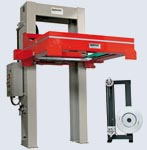
\includegraphics[width=.3\linewidth]{Figures/m1.png}}
    \qquad
    \subfloat[]{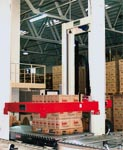
\includegraphics[width=.3\linewidth]{Figures/m2.png}}
    \qquad
    \subfloat[]{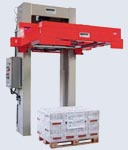
\includegraphics[width=.3\linewidth]{Figures/m3.png}}
    \qquad
    \subfloat[]{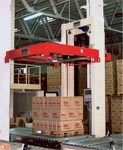
\includegraphics[width=.3\linewidth]{Figures/m4.png}}
    \caption{Горизонтальные автоматические обвязочные машины OR 60}
    \label{fig:or60}
\end{figure}

\subsection*{Вертикальные автоматические обвязочные машины}

\textbf{VR80} --- автоматическая вертикальная стреппинг машина, оборудована стреппинг-головкой MS300 (патент Messersi). Машина VR80 предназначена для вертикального обмотки товара любого типа и размера. Низкий выдвигающийся канал (меч) позволяет пропускать стреп-ленту через низ палеты, таким образом надежно закрепляя товар на палете. 

Во время натяжения ленты, в целях создания одинакового натяжения по всем четырем углам, стреппинг головка двигается поперек, достигая, таким образом, стабильности упаковки.

Программное обеспечение позволяет применить 1, 2, 3 или более количество обмоток стреппинг лентой, в зависимости от потребностей клиента.

\begin{figure}[ht]
    \subfloat[]{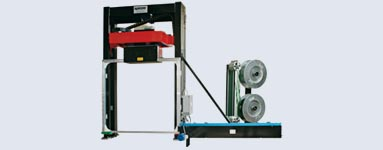
\includegraphics[width=.4\linewidth]{Figures/vr80.png}}
    \qquad
    \subfloat[]{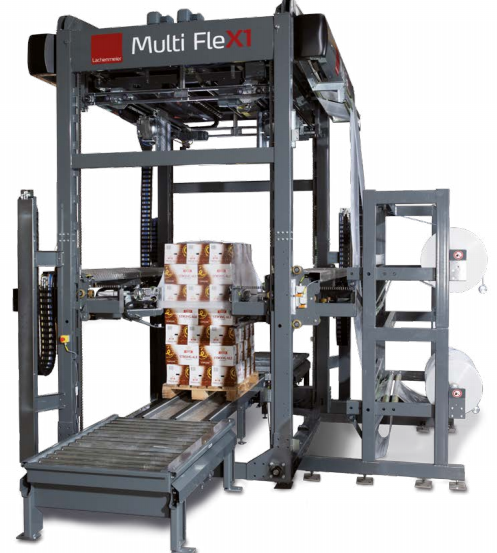
\includegraphics[width=.4\linewidth]{Figures/x1.png}}
    \caption{Машина (а) вертикальная автоматическая обвязочная VR80; (б) стрейч-худ Lachenmeier Multi X1}
    \label{fig:vr80x1}
\end{figure}

Cтретч-худ технология упаковки основана на максимальном использовании эффекта возвратной деформации плёнки. Эта технология имеет существенные преимущества в сравнении с другими методами упаковки палет --- от снижения расхода пленки и энергии до повышения уровня конкурентоспособности продукции. Стретч-худ машина обеспечивает защиту груза с 5 сторон со снижением риска его повреждения в результате воздействия загрязнений и погодных условии, а также обеспечивает защиту от деформации во время транспортировки и хранения

Упаковочная машина Multi FleX1 является высоко универсальной, так как на одной машине можно произвести упаковку палет с разными по размеру грузами. Универсальность заключается в системе захватов где каждый из 4х захватов регулируется индивидуально, тем самым адаптируясь к фактическому размеру груза. Машина способна обматывать палеты размером от 400х400 до 1400х1400 мм. Стрейч-худ машина Lachenmeier Multi Fle X1 обладает, пожалуй, самой большой производительностью --- более чем 250 палет в час.

\section{Технологический процесс упаковки поддонов с плиткой}

Линия упаковки состоит из трёх участков упаковки и автоматической машины, которая доставляет и снимает продукцию с конвейера. Автоматическая машина работает по заданному маршруту, который задаётся в программе. Также машина автоматически расставляет продукцию на складе, присваивая каждому поддону идентификационный номер и сохраняя его в программе. Линия упаковки состоит из горизонтальной, вертикальной обвязки и оборудование для упаковки в стрейч-худ пленку. Продукция для упаковки может быть различной, что делает данную линию гибкой. Главное чтобы продукция соответствовала габаритам для работы на данном оборудовании, указанных заводом изготовителем. В зависимости от процесса упаковки, мы можем исключать любую из машин из работы.

Автоматическая машина привозит палету на роликовый конвейер. Палета начинает движение и останавливается на обвязочной машине, количество обвязок и расположение их на палете задаётся в программе обвязки. Далее палета перемещается на вертикальную обвязку, где в зависимости от заданных параметров, параметры идентичны как на горизонтальной обвязке, происходит обвязка палеты. Далее палета приезжает для упаковки в стрейч-худ плёнку. Комплекс оборудования для упаковки готовых палет в стрейч-худ (stretch hood) пленку включает модуль размотки рулона рукавной пленки, механизм захвата с раскрытием капюшона, вертикальный каркасный лифт для надевания капюшона пленки на палет с готовой продукцией, каркас стрейч-худер а, рольганги для проката поддонов в машине, блок управления и электрический шкаф. Когда палета приезжает плёнка подаётся в механизм захвата, после чего отсчитывается нужная длина плёнки спаивается и обрезается. После чего плёнка одевается на палету с продукцией. В стретч-худ машине пленка растягивается механически и надевается на груз без нагрева. А из этого следует, что нет необходимости использовать газ для нагрева пленки, что так же позволяет эксплуатировать это оборудование во взрывоопасной зоне или на взрывоопасном объекте и удобно для упаковки любого вида продукции. Кроме всего прочего у стретч-худ машин есть положительная особенность --- ввиду отсутствия высокой температуры во время функционирования увеличивается надежность механизмов, способствующая их долговечности и как следствие уменьшению затрат на запасные части и ремонт. После процесса упаковки автоматическая машина забирает палету с конвейера и доставляет на склад.

Алгоритм работы системы показан на листе 2.

\section{Используемое оборудование}

Для перемещения поддонов на конвейер используются автоматические электрические транспортные средства с системой лазерного позиционирования <<LGV>>~\cite{system:logistics}.

<<LGV>> --- это автоматические электрические транспортные средства с системой лазерного позиционирования для перемещения грузов на территории производственных участков, таких как участки складирования или завершения производственного цикла. Они оснащены вилочными захватами и могут перемещать один или несколько поддонов, контейнеров, ящиков или других грузовых единиц.

Внедрение <<LGV>> позволило исключить труд операторов на многих участках. В сочетании с другими полностью автоматизированными системами это дало возможность полностью исключить труд людей в многих зонах складских комплексов. Высокая скорость работы и безопасность перемещения груза между заданными позициями, полная синхронизация работы и интеграция с остальными системами позволяют говорить о том, что <<LGV>> являются самыми современными системами перемещения грузов внутри складского комплекса.

Позиционирование при перемещении транспортного средства осуществляется лазером. Лучи лазера отображаются от особых экранов, которые установлены под потолком складского помещения. Луч лазера, непрерывно контролируя траекторию движения и положение транспортного средства.

Современная система безопасности определяет наличие неподвижных и движущихся объектов на пути движения и немедленно останавливает транспортировщик при появлении неожиданного препятствия. Передвижение каждого отдельного транспортировщика координируется (с использованием радиоканала связи) одним <<наземным>> удаленным компьютером. Этот компьютер осуществляет обмен данными с каждым транспортировщиком и планирует каждое задание, назначая его отдельным машинам, в зависимости от условий движения на складе, степени загруженности транспортировщика или заряда аккумулятора. При необходимости или в случае неполадки Транспортировщики <<LGV>> могут использоваться как обычные электрические погрузчики, которыми управляет оператор с помощью рулевого устройства.

Транспортировщики <<LGV>> с вилочным захватом универсальны, т. к. могут осуществлять сбор и размещение большего количества грузовых единиц одновременно как на уровне земли, так и на различной высоте. Транспортировщики непосредственно подключены к системе управления всем складским комплексом и работают в полном согласовании с другими автоматизированными системами.

Транспортировщик может поставляться в двух вариантах. Первый вариант предназначен для перевозки контейнеров, а второй вариант предназначен для перевозки поддонов, используемых в автоматизированных складах. При необходимости транспортировщик может быть изготовлен из нержавеющей стали, что позволит использовать данное оборудование в таких отраслях, как пищевая промышленность.

\subsection*{Технические характеристики}

Транспортировщики с лазерным управлением (LGV) комплектуются свинцовыми аккумуляторами. Контроллер, устанавливаемый на погрузчике, может выполнять следующие функции:

\begin{itemize}
    \item сохранение в памяти всех вариантов пути;
    \item контроль оборудования, установленного на погрузчике;
    \item контроль безопасности;
    \item поддержание по радио постоянной связи с базовой станцией;
    \item диагностика с помощью стационарной системы;
    \item контроль движения в автоматическом и полуавтоматическом режиме, а также выполнение погрузочно-разгрузочных операций.
\end{itemize}

Транспортировщик комплектуется автоматическим или полуавтоматическим зарядным устройством, подключаемым к сети переменного тока в 380 В.

\begin{figure}[ht]
    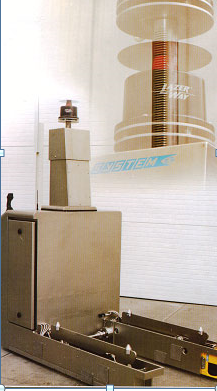
\includegraphics[width=.3\linewidth]{Figures/charging.png}
    \caption{Зарядка транспортировщика <<LGV>>}
    \label{fig:charging}
\end{figure}

Радиостанция устанавливается в специальном корпусе, отвечающим стандарту безопасности IP 55, и выполняет следующие функции:

\begin{itemize}
    \item взаимодействие с базовой станцией посредством стандартных протоколов;
    \item контроль движения с учетом перемещения других транспортных средств;
    \item оптимизация транспортировки;
    \item диагностика;
    \item автоматический учет новых транспортных средств, появляющихся в системе.
\end{itemize}

При необходимости к радиостанции может быть подключен пульт оператора.

Преимущества позиционирования лазером:

\begin{enumerate}
    \item Не требуется монтаж конструкций: учитывая то, что система позиционируется лазером, нет необходимости создавать специальное напольное покрытые или устанавливать дополнительные конструкции.
    \item Простота смены планировки: планировка помещения может быть с легкостью изменена. Так, не надо использовать дополнительное оборудование, все изменения маршрута вносятся непосредственно в программу. Кроме того, система может быть переведена в ручной режим.
    \item Возможность пересечения маршрутов: маршруты движения тележек с лазерным управлением могут соприкасаться или пересекаться, и это не является опасным для данных систем.
    \item Возможность моделирования процесса: благодаря продвинутым технологиям моделирования, существует возможность создания на компьютере модели выполнения работ в тех или иных условиях, что позволяет просчитать все возможные траектории движения и необходимое количество погрузчиков для оптимизации всего процесса работы.
    \item Универсальность: системы с лазерным управлением могут использоваться как для перевозки контейнеров, так и для перевозки поддонов. Простота конструкции и эффективность систем лазерного управления делают данные транспортировщики исключительно универсальными, таким образом, их можно использовать в разных отраслях.
    \item Высокая надежность и безопасность: система контроля движения, установленная на транспортировщике, надежна на 100\%, при этом система безопасности немедленно остановит транспортировщик в случае возникновения неожиданного препятствия.
    \item Малый уровень шума: Очень малый уровень шума достигается за счет использования в транспортировщиках электропривода с аккумуляторной батареей, а также за счет отказа от использования дополнительных элементов (направляющих и т. п.), при контакте с которыми возникает шум.
    \item Новые модификации.
\end{enumerate}

\begin{figure}[ht]
    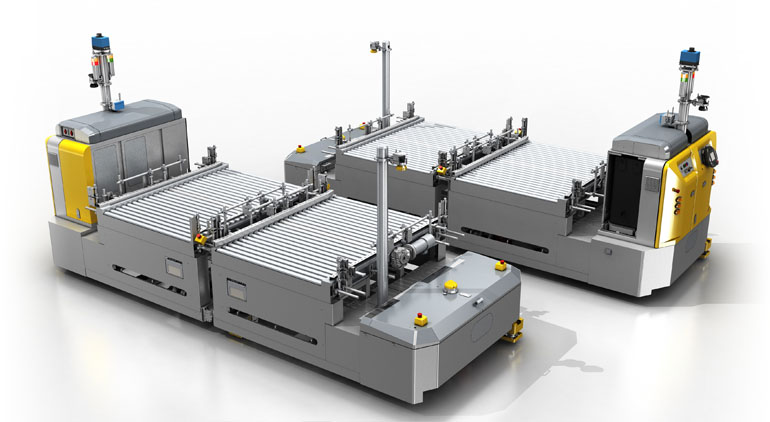
\includegraphics[width=.7\linewidth]{Figures/lgvtrans.png}
    \caption{Транспортировщик LGV Pallet handling}
    \label{fig:lgvtrans}
\end{figure}

Транспортировщики последней версии с лазерным управлением полностью изготовлены из стали, что, помимо прочих преимуществ, дает возможность мыть погрузчик водой. Это играет особенную роль при использовании данных агрегатов в таких отраслях, как, например, пищевая промышленность.

Универсальность данных устройств доказывается тем, что они все чаще и чаще начинают применяться в различных сферах. Их использование совместно с системой управления производственным складом является очень выгодным решением, так это позволяет рационализировать перемещение компонентов продукта, сокращая время ожидания.

Для перемещения панелей к роботу и к устройству подачи поддона используется ленточный конвейер. Он оснащен электродвигателем с редуктором и блоком согласования с контроллером системы управления.

\begin{figure}[ht]
    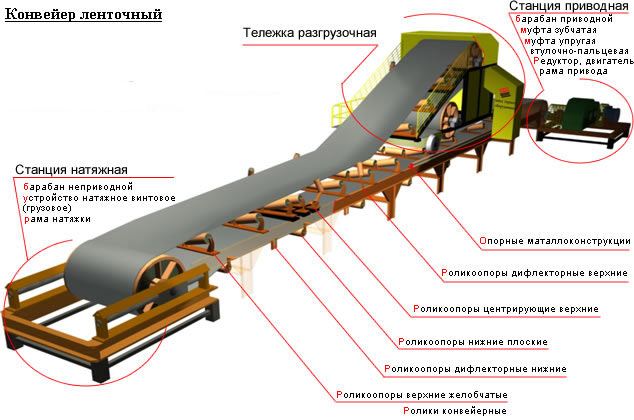
\includegraphics[width=.9\linewidth]{Figures/lent.png}
    \caption{Ленточный конвейер}
    \label{fig:lent}
\end{figure}

Для хранения изготовленной продукции используется автоматический склад. 

Планировка системы показана на листе 1.

\section{Информационная система}

Различают три класса датчиков:

\begin{itemize}
    \item аналоговые датчики, т. е. датчики, вырабатывающие аналоговый сигнал, пропорционально изменению входной величины;
    \item цифровые датчики, генерирующие последовательность импульсов или двоичное слово;
    \item бинарные (двоичные) датчики, которые вырабатывают сигнал только двух уровней: <<включено/выключено>> (иначе говоря, 0 или 1); получили широкое распространение благодаря своей простоте.
\end{itemize}

Требования, предъявляемые к датчикам:

\begin{itemize}
    \item однозначная зависимость выходной величины от входной;
    \item стабильность характеристик во времени;
    \item высокая чувствительность;
    \item малые размеры и масса;
    \item отсутствие обратного воздействия на контролируемый процесс и на контролируемый параметр;
    \item работа при различных условиях эксплуатации;
    \item различные варианты монтажа.
\end{itemize}

\textbf{Контактные датчики} --- это простейший вид резисторных датчиков, которые преобразуют перемещение первичного элемента в скачкообразное изменение сопротивления электрической цепи. С помощью контактных датчиков измеряют и контролируют усилия, перемещения, температуру, размеры объектов, контролируют их форму и т. д. К контактным датчикам относятся путевые и концевые выключатели, контактные термометры и так называемые электродные датчики, используемые в основном для измерения предельных уровней электропроводных жидкостей.

Контактные датчики могут работать как на постоянном, так и на переменном токе. В зависимости от пределов измерения контактные датчики могут быть одно предельными и многопредельными. Последние используют для измерения величин, изменяющихся в значительных пределах, при этом части резистора R, включенного в электрическую цепь, последовательно закорачиваются. 

Недостаток контактных датчиков --- сложность осуществления непрерывного контроля и ограниченный срок службы контактной системы. Но благодаря предельной простоте этих датчиков их широко применяют в системах автоматики.

\textbf{Индуктивные датчики} служат для бесконтактного получения информации о перемещениях рабочих органов машин, механизмов, роботов и т. п. и преобразования этой информации в электрический сигнал.

Принцип действия индуктивного датчика основан на изменении индуктивности обмотки на магнитопроводе в зависимости от положения отдельных элементов магнитопровода (якоря, сердечника и др.). В таких датчиках линейное или угловое перемещение X (входная величина) преобразуется в изменение индуктивности (L) датчика. Применяются для измерения угловых и линейных перемещений, деформаций, контроля размеров и т. д.

В простейшем случае индуктивный датчик представляет собой катушку индуктивности с магнитопроводом, подвижный элемент которого (якорь) перемещается под действием измеряемой величины.

Индуктивный датчик распознает и соответственно реагирует на все токопроводящие предметы. Индуктивный датчик является бесконтактным, не требует механического воздействия, работает бесконтактно за счет изменения электромагнитного поля.


\textbf{Емкостные датчики} --- принцип действия основан на зависимости электрической емкости конденсатора от размеров, взаимного расположения его обкладок и от диэлектрической проницаемости среды между ними.

Емкостные датчики, также как и индуктивные, питаются переменным напряжением (обычно повышенной частоты --- до десятков мегагерц). В качестве измерительных схем обычно применяют мостовые схемы и схемы с использованием резонансных контуров. В последнем случае, как правило, используют зависимость частоты колебаний генератора от емкости резонансного контура, т. е. датчик имеет частотный выход.

Достоинства емкостных датчиков --- простота, высокая чувствительность и малая инерционность. Недостатки --- влияние внешних электрических полей, относительная сложность измерительных устройств.

Емкостные датчики применяют для измерения угловых перемещений, очень малых линейных перемещений, вибраций, скорости движения и т. д., а также для воспроизведения заданных функций (гармонических, пилообразных, прямоугольных и т. п.).


\textbf{Оптические (фотоэлектрические) датчики} --- различают аналоговые и дискретные оптические датчики. У аналоговых датчиков выходной сигнал изменяется пропорционально внешней освещенности. Основная область применения – автоматизированные системы управления освещением.

Датчики дискретного типа изменяют выходное состояние на противоположное при достижении заданного значения освещенности. 

Фотоэлектрические датчики могут быть применены практически во всех отраслях промышленности. Датчики дискретного действия используются как своеобразные бесконтактные выключатели для подсчета, обнаружения, позиционирования и других задач на любой технологической линии.

Оптический бесконтактный датчик, регистрирует изменение светового потока в контролируемой области, связанное с изменением положения в пространстве каких-либо движущихся частей механизмов и машин, отсутствия или присутствия объектов. Благодаря большим расстояниям срабатывания оптические бесконтактные датчики нашли широкое применение в промышленности и не только.

Оптический бесконтактный датчик состоит из двух функциональных узлов, приемника и излучателя. Данные узлы могут быть выполнены как в одном корпусе, так и в различных корпусах. 

По методу обнаружения объекта фотоэлектрические датчики подразделяются на 4 группы:

\begin{enumerate}
    \item Пересечение луча --- в этом методе передатчик и приемник разделены по разным корпусам, что позволяет устанавливать их напротив друг друга на рабочем расстоянии. Принцип работы основан на том, что передатчик постоянно посылает световой луч, который принимает приемник. Если световой сигнал датчика прекращается, в следствии перекрытия сторонним объектом, приемник немедленно реагирует меняя состояние выхода.
    \item Отражение от рефлектора --- в этом методе приемник и передатчик датчика находятся в одном корпусе. Напротив датчика устанавливается рефлектор (отражатель). Датчики с рефлектором устроены так, что благодаря поляризационному фильтру они воспринимают отражение только от рефлектора. Это рефлекторы, которые работают по принципу двойного отражения. Выбор подходящего рефлектора определяется требуемым расстоянием и монтажными возможностями. Посылаемый передатчиком световой сигнал отражаясь от рефлектора попадает в приемник датчика. Если световой сигнал прекращается, приемник немедленно реагирует, меняя состояние выхода.
    \item Отражение от объекта --- в этом методе приемник и передатчик датчика находятся в одном корпусе. Во время рабочего состояния датчика все объекты, попадающие в его рабочую зону, становятся своеобразными рефлекторами. Как только световой луч отразившись от объекта попадает на приемник датчика, тот немедленно реагирует, меняя состояние выхода.
    \item Фиксированное отражение от объекта -принцип действия датчика такой же как и у <<отражение от объекта>> но более чутко реагирующий на отклонение от настройки на объект. Например, возможно детектирование вздутой пробки на бутылке с кефиром, неполное наполнение вакуумной упаковки с продуктами и т. д. 
\end{enumerate}

По своему назначению фотодатчики делятся на две основные группы: датчики общего применения и специальные датчики. К специальным, относятся типы датчиков, предназначенные для решения более узкого круга задач. К примеру, обнаружение цветной метки на объекте, обнаружение контрастной границы, наличие этикетки на прозрачной упаковке и т. д.

Задача датчика обнаружить объект на расстоянии. Это расстояние варьируется в пределах 0,3мм--50м, в зависимости от выбранного типа датчика и метода обнаружения~\cite{gordin:automatics}~\cite{gustav:digital}.

Так как контактные датчики быстро изнашиваются и существуют сложности в установке, а емкостные и индуктивные датчики обладают малой чувствительностью на больших расстояниях, то мы будем использовать оптические датчики фирмы Banner~\cite{tur:optical} отражательные S90U.

\begin{figure}[ht]
    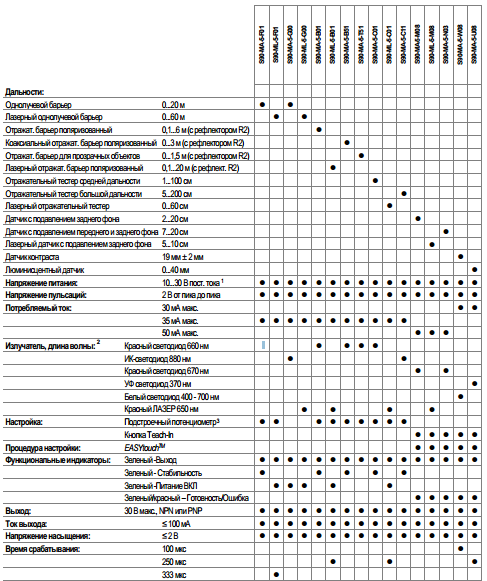
\includegraphics[width=1\linewidth]{Figures/params.png}
    \caption{Параметры отражательного датчика}
    \label{fig:params}
\end{figure}

Подключение данных датчиков к программируемому логическому контроллеру можно производить без использования преобразователей сигнала.

Расположение датчиков показано на листе 1. 

\section{Система управления}

Программируемый логический контроллер (ПЛК) --- специализированное микропроцессорное устройство со встроенным аппаратным и программным обеспечением, которое используется для выполнения функций управления технологическим оборудованием. Прародителями ПЛК были релейные схемы автоматики. Это <<родство>> до сих пор проявляется в виде жесткой цикличности выполнения программы и своеобразного языка программирования. ПЛК --- устройство, доступное для программирования неспециалисту в области информатики и предназначенное для управления последовательными логическими процессами в условиях промышленной среды в реальном масштабе времени. ПЛК циклически опрашивает входы, к которым подключены выключатели, датчики и т. д., и в зависимости от их состояния («включено» --- 1, «выключено» --- 0), включает/выключает выходы, а следовательно и подключенные к выходам исполнительные механизмы. Функциональная схема системы управления (СУ) на базе контроллера показана на рисунке~\ref{fig:fplc}. Используя программное обеспечение, пользователь имеет возможность программировать контроллер или вносить изменения в уже существующую программу.

\begin{figure}[ht]
    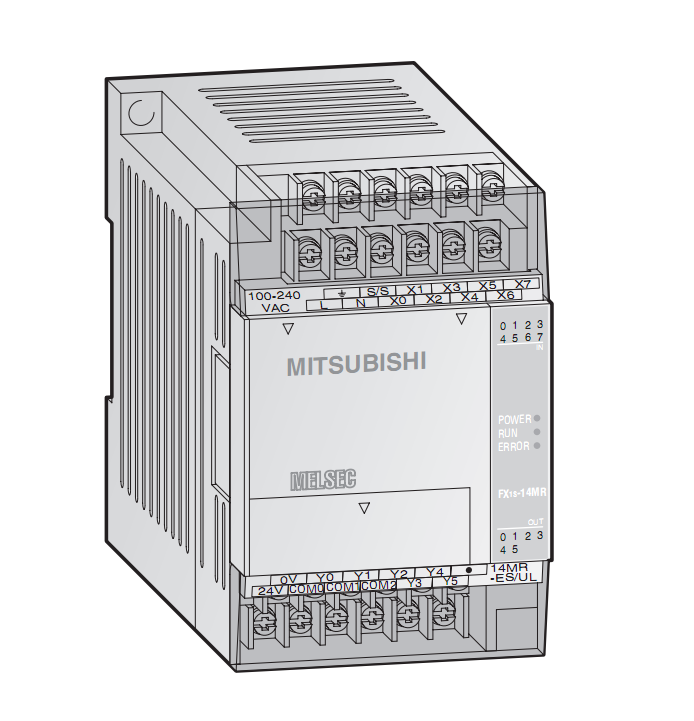
\includegraphics[width=.45\linewidth]{Figures/plc.png}
    \caption{Внешний вид ПЛК}
    \label{fig:plc}
\end{figure}

\begin{figure}[ht]
    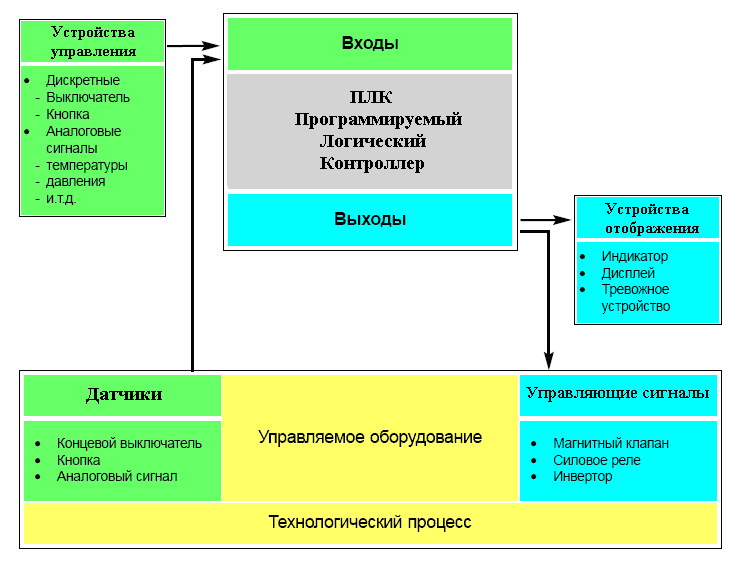
\includegraphics[width=.6\linewidth]{Figures/fplc.png}
    \caption{Функциональная схема ПЛК}
    \label{fig:fplc}
\end{figure}

В нашей системе будем использовать контроллер Mitsubishi серии MELSEC FX1S-30~\cite{labs}.

\begin{figure}[ht]
    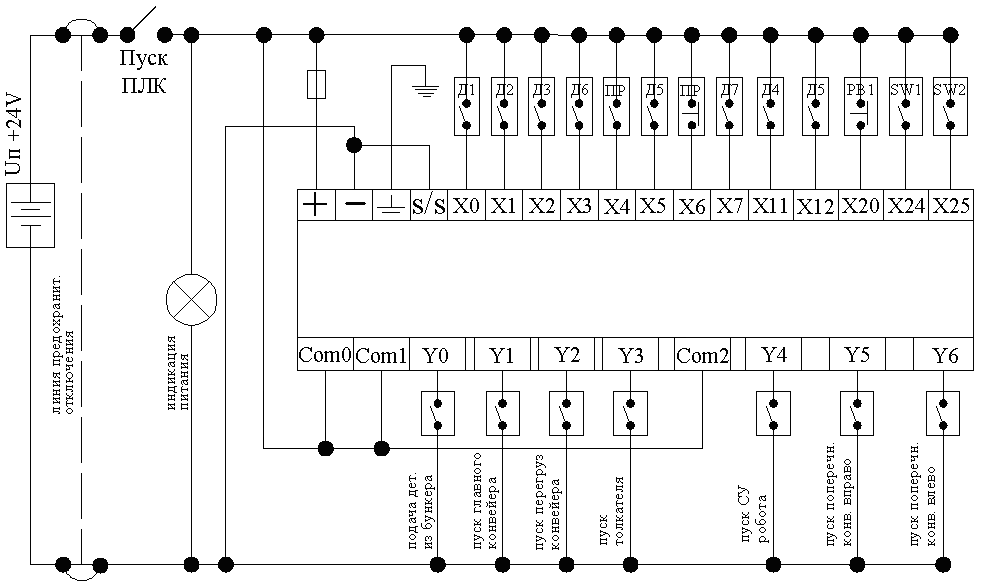
\includegraphics[width=.6\linewidth]{Figures/conjunctions.png}
    \caption{Схема подключения ПЛК FX1S к источнику питания и технологическому оборудованию}
    \label{fig:conjunctions}
\end{figure}

Структурная схема соединения ПЛК с технологическим оборудованием показано на листе 3.

\section*{Заключение}
\addcontentsline{toc}{section}{Заключение}

В ходе курсового проекта был спроектирован участок упаковки поддонов с крепежными элементами. Из совокупности современного оборудования было выбрано то, что наиболее удовлетворяет требованиям технологического процесса. В качестве информационной системы выбраны оптические датчики. Так как система не требует большой вычислительной мощности, то был выбран ПЛК. Составлен алгоритм работы системы и предложена программа.

\bibliography{../web,../books}
